%%%%%% Krav %%%%%%
\chapter{Krav}
\vspace{-0.5cm}
I dette afsnit beskrives kravene til projektet. Indledningsvis præsenteres de funktionelle krav  ved brug af use cases. På figur \ref{fig:useCaseDiagram} vises et use diagram der viser use cases tilhørende systemet. Efter use case diagrammet følger en kort beskrivelse af de seks use cases og deres funktion. Afsnittet sluttets af med ikke-funktionelle krav, der er både er krav til systemet som helhed og til systemets blokke.

En mere detaljeret beskrivelse af kravene findes i projektets kravspecifikation[x] .
\vspace{-0.3cm}

\section{Funktionelle krav}
\vspace{-0.2cm}
Til systemet er der identificeret de 2 aktører: Bruger \& GPS-satellit. Bruger er primær aktør der ønsker at initialisere og styre systemet. Bruger er ansvarlig for at oprette flyveopsætninger på webapplikationen og tilslutte batteri til dronen.
GPS-satellitter er en sekundær aktør, der gør det muligt for dronen at finde egen position. 

På figur \ref{fig:useCaseDiagram} vises et use case diagram. Diagrammet viser systemets aktørerne og i hvilke use cases aktørerne optræder. 
\begin{figure}[H]
	\centering
	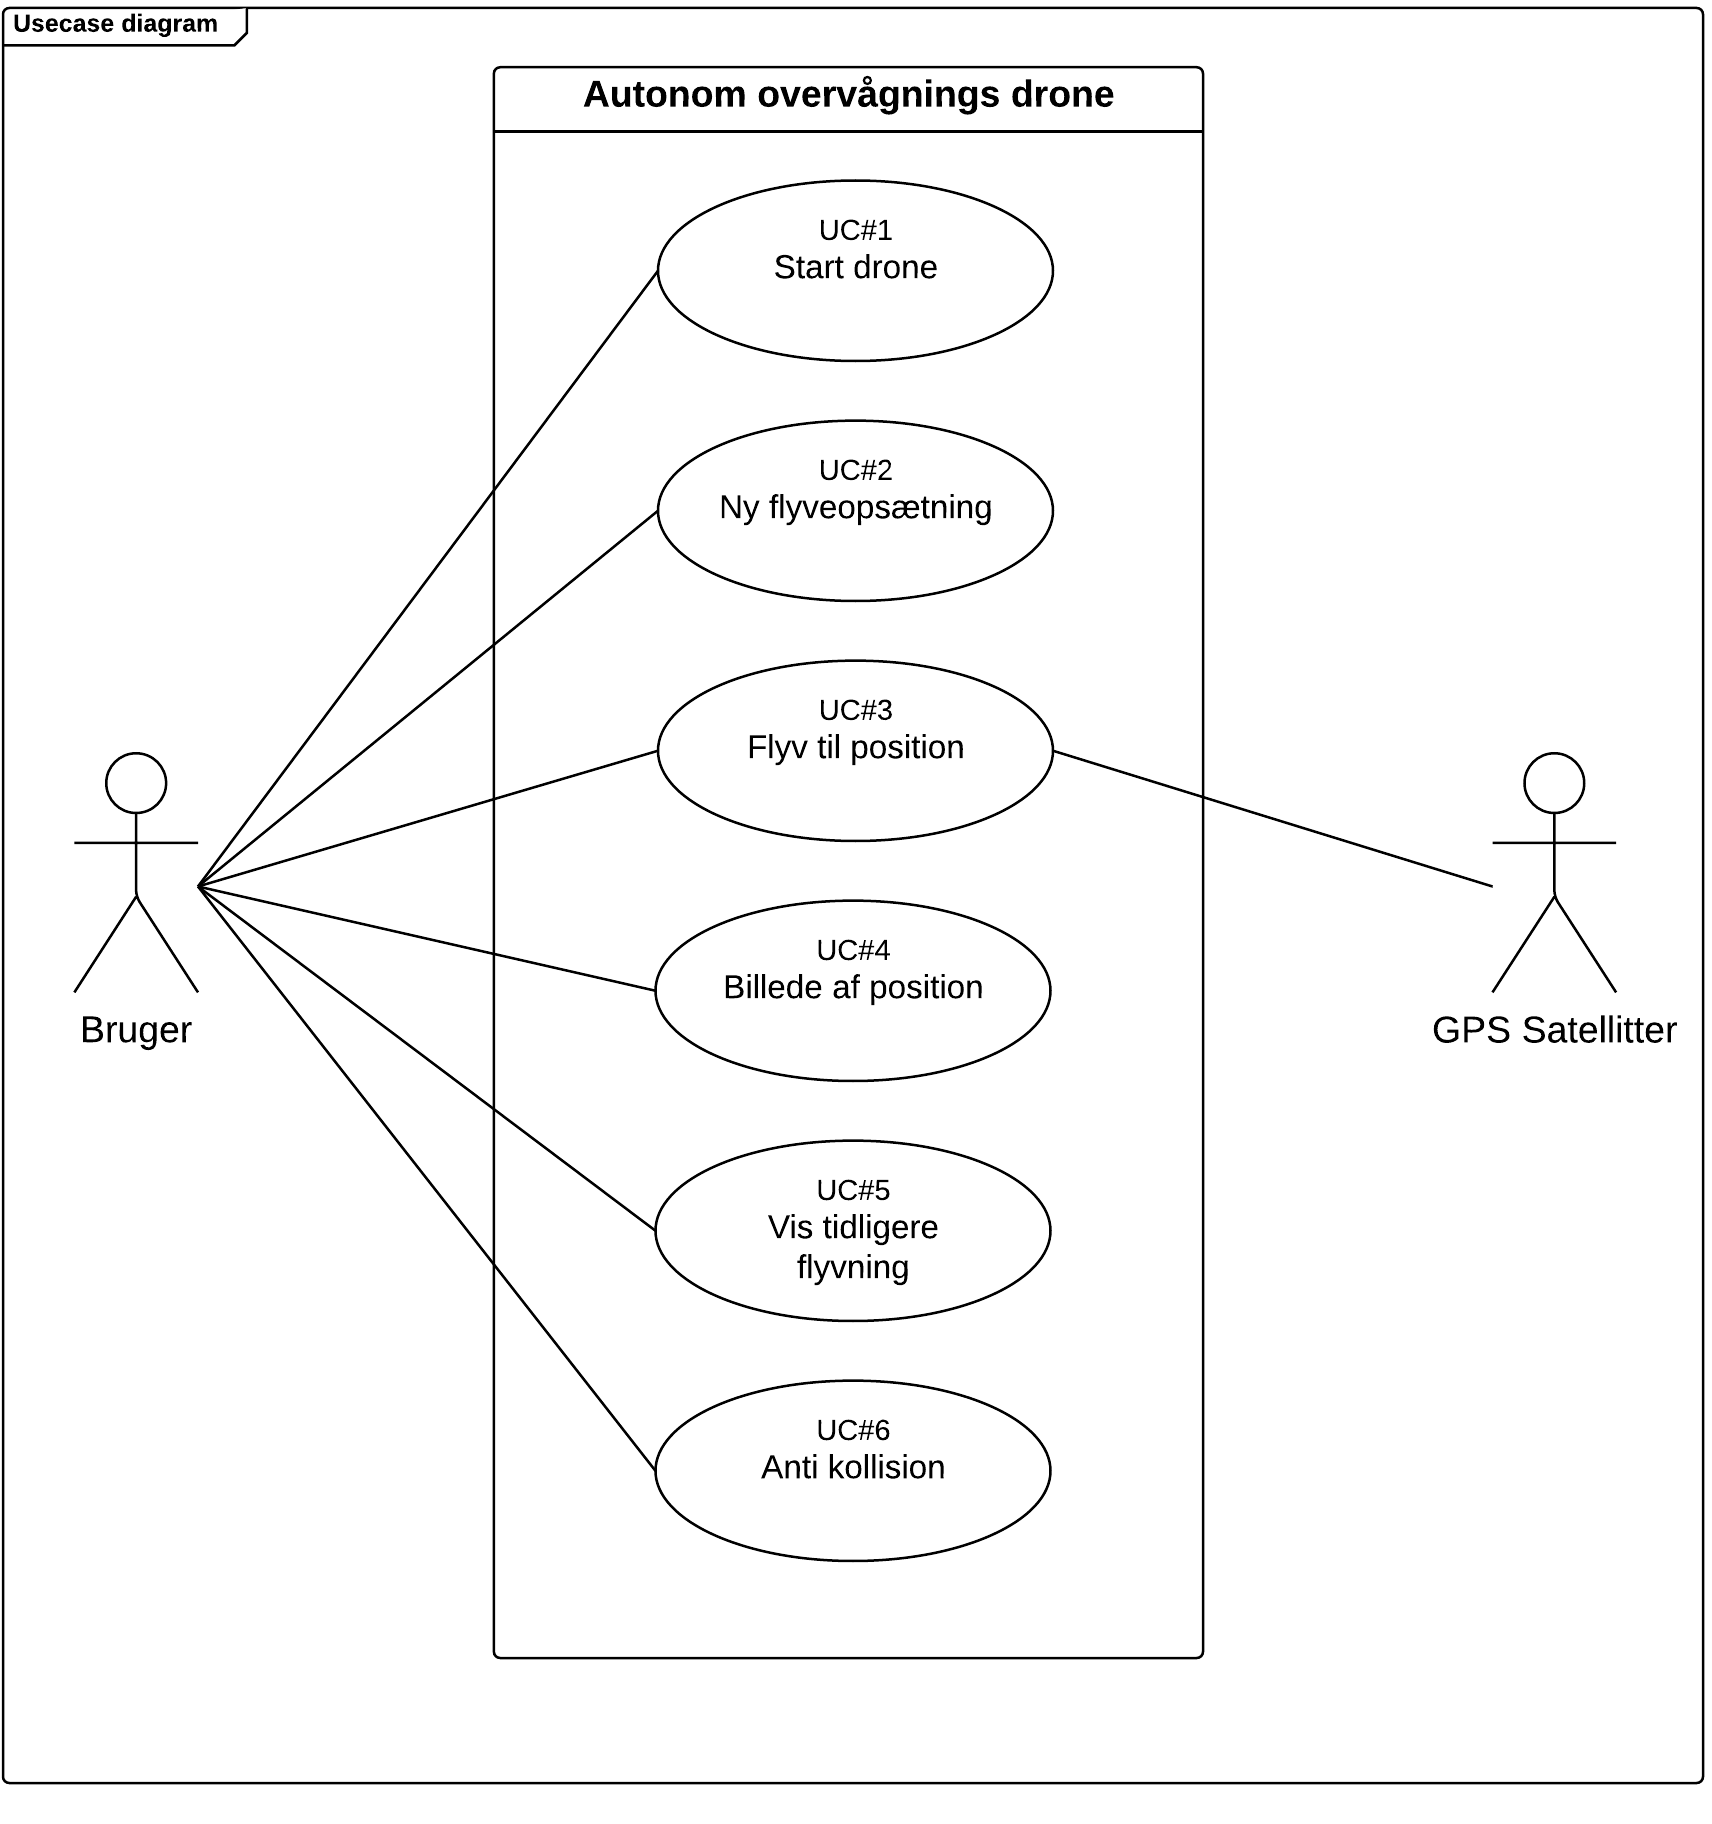
\includegraphics[width=0.65\textwidth]{Billeder/Krav/Use_case_diagram}
	\vspace{-0.3cm}	
	\caption{Use case diagram}
	\label{fig:useCaseDiagram}
\end{figure}

Alle use cases er beskrevet som fully dressed use cases i projektets kravspecifikation. 
I fully dressed use cases beskrives hvordan hovedforløb ser ud i en given use case, hvis den succesfuld gennemføres. Desuden beskrives startbetingelse, aktører og tilføjelser.

Nedenfor vises beskrivelser af hovedforløb og funktion af de seks use cases:\\

\textbf{Use case 1: Start drone} \\
Bruger tilslutter batteri til drone og dronen initialiseres. Drone sender information om nuværende position til server.\\

\textbf{Use case 2: Ny flyveopsætning} \\
Bruger logger på webapplikation og opretter en ny flyveopsætning. Flyveopsætningen sættes tilgængelig for drone på server.\\

\textbf{Use case 3: Flyv til position}\\
Drone henter flyveopsætningen fra server og påbegynder flyvning. Under flyvning tilpasser drone  løbende flyvehøjde og flyveorientering og fortsætter flyvning mod ønsket position. \\

\textbf{Use case 4: Billede af position} \\
Når drone er ankommet til ønsket GPS position og tages et billede. Hvis billedet accepteres, flyver dronen videre mod næste GPS koordinat eller til udgangsposition. \\

\textbf{Use case 5: Vis tidligere flyvninger} \\
Bruger tilgår webapplikation for at se flyveruter og billeder tidligere flyvninger.\\

\textbf{Use case 6: Anti kollision} \\
Drones anti kollisions sensorer bruges til at detekterer forhindringer. I tilfælde af forhindringer ændre drone enten flyveretning eller flyvehøjde for at undgå kollision. \\



\section{Ikke-funktionelle krav}

De ikke-funktionelle krav opstilles ud fra systemspecifikationerne og er krav som ikke kan defineres i use cases. De ikke-funktionelle krav har ingen indvirkning på systemets endelig funktion, kun systemspecifikationer.  

De generelle krav, er krav der omhandler både drone, server og webapplikation, altså krav der ikke kan placeres i en specifik gruppe. For at sikre at dronen performans, er der eksempelvis opsat krav til de forskellige moduler og sensorer der er monteret på dronen. 
